\usetikzlibrary{arrows.meta}
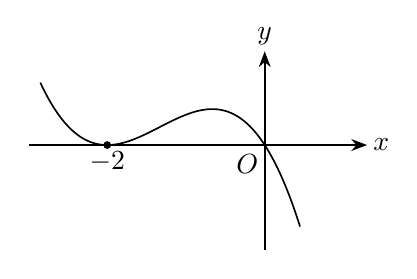
\begin{tikzpicture}[x=1cm,y=0.7cm,line width=.6pt,>=Stealth,font=\normalsize]
\coordinate (O) at (0,0);
\coordinate (T) at (-2,0);
\draw[->] (-3.0,0)--(1.3,0) node[right,inner sep=0pt,xshift=2pt] {$x$};
\draw[->] (0,-1.9)--(0,1.7) node[above,inner sep=0pt,yshift=2pt] {$y$};
\draw[domain=-2.85:0.45,samples=161] plot (\x,{-0.55*\x*(\x+2)*(\x+2)});
\fill (T) circle (1.4pt);
\node[below,inner sep=0pt,yshift=-2pt] at (T) {$-2$};
\node[below left,inner sep=0pt,xshift=-2pt,yshift=-3pt] at (O) {$O$};
\end{tikzpicture}
